
\title{Riepilogo Reti di Calcolatori}
\author{Jacopo Nasi\\
        Ingegneria Informatica\\
        Politecnico di Torino}
\date{I Periodo - 2016}

\documentclass[12pt]{article}
\usepackage[utf8]{inputenc}
\usepackage{geometry}
\usepackage{mathtools}
\usepackage{graphicx}
% Misure Documento
\geometry{ a4paper, total={170mm,257mm},left=35mm, right=35mm, top=35mm, bottom=35mm }

\begin{document}

\begin{figure}
  \centering
  
\includegraphics[width=10cm]{images/polito.pdf}
\end{figure}

\maketitle
\newpage
\tableofcontents
\newpage
``The most compelling reason for most people to buy a computer for the home will be to link it to a nationwide communications network. We’re just in the beginning stages of what will be a truly remarkable breakthrough for most people– –as remarkable as the telephone.''\\
\rightline{{\rm --- Steve Jobs, Feb. 1th 1985}}
\newpage
\section{Struttura}
\subsection{Concetti Generali}\label{subsubsec}
Introduzione alle Reti di Calcolatori dal punto di vista strutturale.
\subsubsection{Definizioni}
La maggior parte delle definizioni derivano dal "Blue Book" del CCITT o IUT-T oggi.\\
\begin{itemize}
  \item \textbf{Comunicazione}: Trasferimento di informazioni secondo convenzioni prestabilite.\\
  \item \textbf{Telecomunicazione}: Qualsiasi trasmissione e ricezione di segnali che rappresentano informazioni di qualsiasi natura, attraverso cavi, radio o altri sistemi ottici e elettromagnetici.\\
  \item \textbf{Servizio di Telecomunicazione}: Ciò che viene offerto da un gestore pubblico o privato ai proprio clienti al fine di soddisfare una specifica esigenza di telecomunicazione.\\
  \item \textbf{Funzioni in una rete di telecomunicazioni}: Operazioni svolte all'interno della reta al fine di offrire i servizi.(es: tutte le fasi di una chiamata: segnalazione, commutazione, trasmissione, ecc...)\\
  \item \textbf{Segnalazione}: Scambio di informazioni che riguardano l'apertura, il controllo e la chiusura di connessioni e la gestione di una rete di telecomunicazione.\\
  \item \textbf{Commutazione}: Il processo di interconnessione tra Unità Funzionali, Canali di Trasmissione e Circuiti di Telecomunicazione per il tempo necessario al trasferimento dei segnali.\\
  \item \textbf{Trasmissione}: Il trasferimento di segnali da un punto a uno o più altri punti.\\
  \item \textbf{Mezzo Trasmissivo}: Mezzo fisico in grado di trasportare segnali tra due o più punti.\\
  \item \textbf{Canale}: Concatenazione di porzioni di mezzi trasmissivi.\\
  In riferimento allo studio di reti telematiche:\\
  \item \textbf{Banda}: Quantità di dati [bit] per unità di tempo [secondi].\\
  \item \textbf{Capacità}: Massima velocità trasmissiva [bit/s] del canale.\\
  \item \textbf{Traffico Offerto}: Quantità di dati per unità di tempo che una sorgente cerca di inviare in rete.\\
  \item \textbf{Traffico Smaltito (Throughput)}: Porzione di traffico offerto che riesce ad essere consegnata correttamente alla destinazione.\\
  Sicuramente questi vincoli vengono rispettati:
  \begin{itemize}
    \item Throughput $\leq$ Capacità Canale
    \item Throughput $\leq$ Traffico Offerto
  \end{itemize}
\end{itemize}
\subsubsection{Topologia}
La topologia rappresenta un insieme di nodi e canali che fornisce un collegamento tra due o più punti per permettere la telecomunicazione tra essi.\\
Prende il nome di \textbf{Nodo} un punto in cui avviene la commutazione, mentre si chiama \textbf{Canale} un mezzo di trasmissione, sia nel caso uni che bi-direzionale.
\paragraph{Tipi di Canale} I canali posso essere di due tipi:
\begin{itemize}
  \item Punto-Punto: Due nodi collegati agli estremi del canale in modo parietico.
  \item Multi-Punto: Più nodi collegati ad un unico canale: un nodo master e numerosi slave.
  \item Broadcast: Singolo canale di comunicazione dove l'informazione inviata viene ricevuta da tutti gli altri. Nel caso in cui i dati contengano l'indirizzo di destinazione realizzo di fatto un P-P.
\end{itemize}
La disposizione di nodi e canali definisce la topologia della rete. Viene definita da un grafo G=(V,A) con V (= insieme di vertici [nodi]) ed A (= insieme degli archi [canali]).\\
Gli argchi possono essere Diretti (Unidirezionali) o Non Diretti (Bidirezionali).\\
Considerando N=$|V|$ e C=$|A|$ le principali topologie sono:
\begin{itemize}
  \item \textbf{Maglia Completa}: C=N(N-1)/2, + molto resistente ai guasti, - troppi canali. Esistono molti percorsi, usata solo con pochi nodi.
  \item \textbf{Albero}: C=N-1, - vulnerabile, + pochi canali. Usata per ridurre i costi e semplificare la stesura dei canali.
  \item \textbf{Stella Attiva}: C=N (centro NON nodo), - vulnerabile, + pochi canali. Complessità demandata al centro stella. Molto usata nelle reti locali.
  \item \textbf{Stella Passiva}: C=1 (anche se N fili), - potenzialmente vulnerabile, + pochi canali. Esiste solo un canale broadcast.
  \item \textbf{Maglia}: N-1 $<$ C $<$ N(N-1)/2, - non regolare, - instradamento complesso, + flessibile in n.can e restistenza. Topologia maggiormente usata.
  \item \textbf{Anello}: Uni (C=N/2) e Bi (C=N) direzionale, usate in reti locali e per topologie magliate, sopravvivenza garantita in bi-dir.
  \item \textbf{Bus}: C=1, semplcità isntrdamento.
\end{itemize}
Si possono distinguere due tipi di topologia, quella fisica e quella logica. La prima tiene conto dei mezzi trasmissivi mentre la seconda definisce le interconnessioni tra nodi mediante canali. Chiaramente la scelta di una topologia influisce direttamente sulle prestazioni della rete. Il traffico smaltibile da una rete dipende dalla media della distanza tra ogni coppia di nodi della rete, pesata dalla quantità di traffico scambiata tra i due nodi. Nel caso di traffico uniforme e topologie regolari il throughput è inversamente proporzionale alla distanza media.

\subsubsection{Servizi di Telecomunicazione}
Un servizio di telecomunicazione è ciò che viene offerto da un gestore pubblico o privato ai propri clienti al fine di soddisfare una specifica esigenza di telecomunicazione.\\
Diretta conseguenza di questa definizione sono i tipi di reti, esse possono essere DEDICATE (singolo servizio: radio, TV) o INTEGRATE (multi servizio: internet).\\
I servizi possono essere classificati in questo modo:
\begin{itemize}
  \item \textbf{Portanti}: Forniscono la possibilità di trasmissione di segnali tra interfacce utente-rete, esempio l'ADSL.
  \item \textbf{Teleservizi}: Forniscono la completa possibilità di comunicazione tra utenti, includendo le funzioni egli apparati di utente secondo protocolli definiti. Esempio: Telefonia, Telefax, Web Browsing.
\end{itemize}
I teleservizi inoltre possono essere di base (posta elettronica), ovvero che garantiscono le minime funzionalità, oppure supplementari con funzionalità aggiuntive a quelle base, spesso vendute separatamente (video-on-demand, mailing list, segreteria telefonica, ecc...).\\
I principali servizi vengono offerti in due modalità, client-server o peer-to-peer e possono essere classificati in diversi modi, vi sono quelli interattivi (conversazionali, messaggistica, consultazione) o diffusivi (con o senza controllo di presentazione dall'utente). Entrambi possono trasferire informazioni trammite molteplici "canali" audio, video o dati.
\paragraph{Client-Server}
Questo tipo di modello prevede due ruoli ben distinti. Il cliente è colui che inizia l'interazione con il server richiedendo un servizio. Il server ha invece il compito di fornire il servizio richiesto al client. Questa è il modello usato dalla maggior parte degli applicativi.\\
I client sono attivati solo nel momento in cui viene richiesto un servizio a differenza dei server che sono sempre disponibili ed in attesa di richieste.
\paragraph{Peer-to-Peer}
Questo modello è stato introdotto nel mondo di internet più recentemente ed è principalmente pensato per le interazioni tra gruppi di utenti dopo tutti gli applicativi sono paritetici ovvero mettono a disposizione informazioni condivise.

\subsubsection{Tipi di trasmissione}
L'informazione può essere condivisa principalmente in due modi, in modo ANALOGICO o in modo NUMERICO (DIGITAL).
\paragraph{Analogico}
La trasmissione viene trasferita per mezzo di un segnale elettrico, di conseguenza sarà continuo, limitato e di infiniti valori. La rappresentazione deriverà dalle variazioni del segnale, ad esempio la trasmissione del segnale audio sul cavo connettore delle cuffie.
\paragraph{Numerica}
Anche in questo caso l'informazione viene trasferita attraverso un segnale elettrico ma esso sarà discontinuo, limitato e con un numero finito di valori. Ad ogni informazione discreta verrà associato un segnale ricostruibile dal ricevitore che ne farà uso.\\
Nelle reti telematiche l'informazione viene trasferita in forma digitale usando segnali analogici e digitali. Nel caso in cui la sorgente si presenti in maniera analogica essa viene preventivamente capionata in modo da porterla trasformare in una controparte digitale. Questo processo potrebbe presentare delle perdite se non vengono rispettate determinate condizioni.\\
Il livello successivo alla caratterizazione del segnale riguardo la sua trasmissione vera e propria che può essere gestita in due modi, SERIALE o PARALLELA. Il principale problema di tutte e due è legato alla sincronizzazione. Questo problema può essere gestito in due modalità, SINCRONA ed ASINCRONA. Ma questo corso non si occupa nello specifico di questi argomenti.

\subsubsection{Condivisione di Canale}
La convisione di canale può essere di due tipologie, si parla di:
\begin{itemize}
  \item \textbf{Multiplazione}: Se tutti i flussi sono disponibili in un unico punto.
  \item \textbf{Accesso Multiplo}: Se i flussi accedono al canale da punti differenti.
\end{itemize}
Per eseguire queste funzioni possono essere usate frequenza, tempo, codice o spazio.
\paragraph{Multiplazione di frequenza FDM-FDMA}
In questa soluzione la separazione viene ottenuta usando bande di frequenza diverse, chiaramente per evitare problemi avremo bisongo di alcune bande di guardia.
\paragraph{Multiplazione di tempo TDM-TDMA}
La separazione in questo caso viene effettuata trammite intervalli di tempo diversi con trame temporali ripetitive. Ovviamente anche in questo caso necessiteremo di tempi di guardia tra un'intervallo e l'altro. Questa soluzione è probabilmente la migliore se le condizioni sono identiche tra tutti gli utenti.
\paragraph{Multiplazione di codice CDM-CDMA}
Questo tipo di divisone si ottiene usando codici differenti che devono essere riconoscibili. Viene ottenuta trammite una sovrapposizione sia in tempo che in frequenza, notare bene come essa non sia un misto delle due, ma una vera e propria sovrapposizione attraverso segnali ortogonali. La trasmissione consiste nel prodotto tra bit di informazione e codice, mentre l'operazione di ricezione equivale ad un prodotto scalare tra vettori. La struttura si presenta discretamente resistente a disturbi.\\
\begin{figure}[h!]
  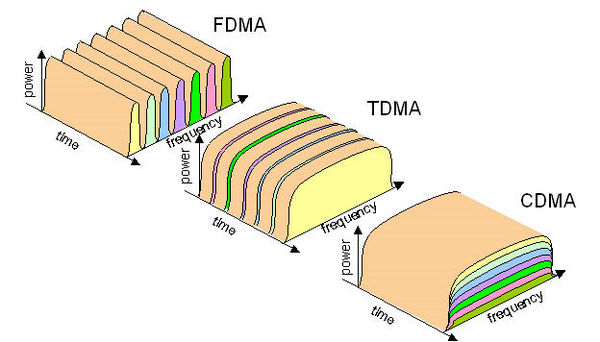
\includegraphics[width=\linewidth]{images/csma.jpg}
  \caption{Channel Multiplation}
  \label{fig:cmult}
\end{figure}
\paragraph{Multiplazione di spazio}
Le reti permettono di sfruttare la diversità spaziale del sistema per far coesistere più flussi di informazione in punti diversi. Questa possibilità può essere sfruttata per aumentare la capacità di una rete.\\
Tutte queste soluzioni possono essere applicate in modo predeterminato o in maniera statistica in modo da permettere una flessibilità relativa alla situazione.

\subsubsection{Commutazione di circuito}
Usata sin dagli albori della telefonia, usa le risorse disponibili per allocare un circuito (collegamento fisico) a ogni richiesta di servizio. Il circuito stabilito rimarrà ad uso esclusivo degli utenti per tutta la durata della loro connessione, le risorse verranno infatti rilasciate solo al termine della comunicazione. L'esempio principe è la rete telefonica.\\
I vantaggi principali sono:
\begin{itemize}
  \item Banda costante garantita.
  \item Ritardi costanti e ridotti.
  \item Trasparenza circuito (formati, velocità e protocolli).
\end{itemize}
Gli svantaggi invece:
\begin{itemize}
  \item Risorse dedicate.
  \item Buona efficenza solo per sorgenti continue.
  \item Tempo di apertura circuito.
  \item Tariffazione in base al tempo di allocazione.
\end{itemize}
Generalmente questa pratica risulta utile solo nel caso in cui il canale allocato risulti completamente sfruttato, altrimenti sarà sicuramente più vantaggioso lo smistamento.
\subsubsection{Commutazione di pacchetto}
L'idea principale di questo tipo di tecnologia è quella di non predeterminare l'allocazione, sopratutto per l'uso esclusivo da parte di due o più utenti. Questa tecnica può essere paragonata al sistema postale.\\
L'informazione da trasferire viene organizzata in unità dati (PDU) che comprendono informazioni di utente e protocollo.
\begin{itemize}
  \item \textbf{PDU:} Protocol Data Unit
  \item \textbf{PCI:} Protocol Control Information
  \item \textbf{SDU:} Service Data Unit
\end{itemize}
La PDU viene spesso chiamata pacchetto (packet) o datagram.\\
Ogni unità dati viene consegnata alla rete. Ogni nodo si occuperà di memorizzare il pacchetto, analizzare e determinare la destinazione del canale ed accodarlo per l'uscita. Questa tecnica prende il nome di \textbf{STORE \& FORWARD}.
\paragraph{Pacchetti}
Per poter funzionare questa tecnica ha bisogno di frazionare le informazioni in molti pacchetti ed essi potranno essere di dimensione fissa o variabile. In merito a questa soluzione vanno valutate alcune questioni riguardanti i vari ritardi nella trasmissione. Infatti in ogni canale in cui è trasmesso il nostro pacchetto subira un ritardo di TX (e di RX) in funzione della dimensione e della velocità della trasmissione ed un ritardo di propagazione in relazione alla lunghezza del canale.\\
Per ogni nodo invece avremo un ritardo di elaborazione ed un ritardo di accodamento (spesso trascurabili). Fortunatamente nella nostra comunicazione potremo sfruttare la parallelizzazione (pipeline) in modo da migliorare l'efficenza del nostro canale.\\
La dimensione dei pacchetti gioca un ruolo fondamentale nella trasmissione, pacchetti più brevi infatti favoriscono la parallelizzazione della trasmissione e diminuiscono la \% di errori, dovrò comunque tenere di conto che per ogni pacchetto avrò la necessità di un header.\\
I vantaggi principali di CAP:
\begin{itemize}
  \item Efficente utilizzo anceh con traffico intermittente.
  \item Possibilità di verifica del percorso.
  \item Conversioni possibili.
  \item Tariffazioni in funzione del traffico emesso.
\end{itemize}
Gli svantaggi sono invece:
\begin{itemize}
  \item Difficoltà ad ottenere garanzie di banda.
  \item Ogni nodo deve elaborare il pacchetto.
  \item Ritardi variabili.
\end{itemize}
Sostanzialmente la prima soluzione privilegia la qualità del servizio al singolo utente, la seconda invece l'efficenza complessiva della rete.\\
\paragraph{Modi di trasferimento}
In commutazione a pacchetto vi sono due principali modi per il trasferiemtno di informazioni. Quella datagram, descritta precedentemente, e quella a circuito virtuale.\\
La seconda soluzione si differenzia per la suddivisione in tre fasi:
\begin{enumerate}
  \item Apertura Connessione (segnalazione)
  \item Trasferiemento Dati
  \item Chiusura Connessione (segnalazione)
\end{enumerate}
Dopo aver stabilitò un'accordo tra i due interlocutori ed il fornitore i pacchetti seguiranno tutti lo stesso percorso a differenza del datagram dove i paccheti potrebbero tranquillamente seguire percorsi differenti. La soluzione a CV rimane comunque differente da quella a commutazione di circuito perchè non vengono allocate staticamente ed esclusivamente delle risorse.

\bibliographystyle{abbrv}
\bibliography{simple}

\end{document}
